\documentclass[aspectratio=169]{beamer}
\usetheme{Madrid}
\usecolortheme{default}

% Packages
\usepackage{amsmath}
\usepackage{amssymb}
\usepackage{graphicx}
\usepackage{tikz}
\usepackage{booktabs}
\usepackage{array}
\usepackage{multirow}
\usepackage{algorithm}
\usepackage{algorithmic}
\usepackage{subcaption}
\usepackage[style=authoryear,backend=biber,maxcitenames=2]{biblatex}
\addbibresource{hybrid_systems_references.bib}

% Custom colors
\definecolor{darkblue}{RGB}{0,51,102}
\definecolor{lightblue}{RGB}{173,216,230}
\definecolor{darkgreen}{RGB}{0,100,0}
\definecolor{orange}{RGB}{255,165,0}

% Title page information
\title[Hybrid System Identification]{Identification of Hybrid Systems: A Tutorial}
\subtitle{Methods, Challenges, and Recent Advances}
\author[Workshop]{Based on \cite{paoletti2007identification} \\ with Recent Developments (2020-2024)}
\institute{Workshop on Automata Learning}
\date{\today}

\begin{document}

% Title slide
\frame{\titlepage}

% Table of contents
\begin{frame}{Outline}
\tableofcontents
\end{frame}

\section{Introduction to Hybrid Systems}

\begin{frame}{What are Hybrid Systems?}
\begin{block}{Definition}
\textbf{Hybrid systems} are heterogeneous dynamical systems whose behavior is determined by interacting continuous and discrete dynamics \cite{paoletti2007identification}.
\end{block}

\begin{columns}[t]
\begin{column}{0.5\textwidth}
\textbf{Continuous dynamics:}
\begin{itemize}
\item Variables from continuous sets
\item Differential/difference equations
\item Traditional control theory
\end{itemize}
\end{column}
\begin{column}{0.5\textwidth}
\textbf{Discrete dynamics:}
\begin{itemize}
\item Variables from finite sets
\item Logic conditions
\item Event-driven behavior
\end{itemize}
\end{column}
\end{columns}

\vspace{0.3cm}
\begin{exampleblock}{Critical CPS Applications}
\vspace{-0.2cm}
\begin{itemize}
\item \textbf{Autonomous vehicles}: Safety verification
\item \textbf{Industrial robotics}: Multi-modal control
\item \textbf{Medical devices}: Critical monitoring
\item \textbf{Smart grids}: Energy management
\item \textbf{Digital twins}: Predictive maintenance
\end{itemize}
\end{exampleblock}
\end{frame}

\begin{frame}{Why Hybrid System Identification?}
\begin{columns}[t]
\begin{column}{0.5\textwidth}
\textbf{Challenges:}
\begin{itemize}
\item First-principles modeling often impossible
\item Complex interactions between continuous and discrete dynamics
\item Discontinuous behaviors
\item Multiple operating modes
\end{itemize}
\end{column}
\begin{column}{0.5\textwidth}
\textbf{Solutions:}
\begin{itemize}
\item Data-driven approaches
\item Automatic model structure detection
\item Parameter estimation from observations
\item Universal approximation properties
\end{itemize}
\end{column}
\end{columns}

\vspace{0.5cm}
\begin{alertblock}{Key Insight - The "Learn-First" Necessity}
The "model-first" imperative in modern Cyber-Physical Systems (CPS) creates a "learn-first" necessity when models are absent. Hybrid system identification provides automated means to learn necessary models from data for formal verification, control design, and digital twin creation.
\end{alertblock}
\end{frame}

\section{Piecewise Affine (PWA) Systems}

\begin{frame}{Piecewise Affine Systems - State Space Form}
\begin{block}{Discrete-time Switched Affine Model}
\begin{align}
x_{k+1} &= A_{\sigma(k)} x_k + B_{\sigma(k)} u_k + f_{\sigma(k)} + w_k \\
y_k &= C_{\sigma(k)} x_k + D_{\sigma(k)} u_k + g_{\sigma(k)} + v_k
\end{align}
\end{block}

Where:
\begin{itemize}
\item $x_k \in \mathbb{R}^n$: continuous state
\item $u_k \in \mathbb{R}^p$: input
\item $y_k \in \mathbb{R}^q$: output
\item $\sigma(k) \in \{1, \ldots, s\}$: discrete state
\item $w_k, v_k$: noise terms
\end{itemize}

\begin{block}{PWA Switching Rule}
$$\sigma(k) = i \quad \text{iff} \quad \begin{bmatrix} x_k \\ u_k \end{bmatrix} \in \Omega_i$$
where $\{\Omega_i\}_{i=1}^s$ is a polyhedral partition of the state-input domain.
\end{block}
\end{frame}

\begin{frame}{PWA Systems - Input-Output Form}
\begin{block}{PWARX Model}
$$y_k = \theta_{\sigma(k)}^T \begin{bmatrix} r_k \\ 1 \end{bmatrix} + e_k$$
\end{block}

Where:
\begin{itemize}
\item $r_k = [y_{k-1}^T \ldots y_{k-n_a}^T \; u_k^T \; u_{k-1}^T \ldots u_{k-n_b}^T]^T$: regression vector
\item $\sigma(k) = i$ iff $r_k \in \mathcal{R}_i$
\item $\{\mathcal{R}_i\}_{i=1}^s$: polyhedral partition of regressor domain
\end{itemize}

\begin{block}{Polyhedral Regions}
$$\mathcal{R}_i = \left\{r \in \mathbb{R}^d : H_i \begin{bmatrix} r \\ 1 \end{bmatrix} \leq 0\right\}$$
\end{block}

\begin{alertblock}{Key Property}
PWA models have universal approximation properties and can represent various hybrid system classes including Mixed Logical Dynamical (MLD), Linear Complementarity (LC), and Hybrid Automata!
\end{alertblock}
\end{frame}

\begin{frame}{PWA Map Visualization}
\begin{center}
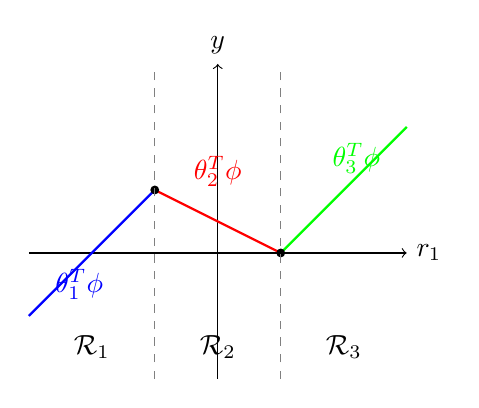
\begin{tikzpicture}[scale=0.8]
% Draw axes
\draw[->] (-3,0) -- (3,0) node[right] {$r_1$};
\draw[->] (0,-2) -- (0,3) node[above] {$y$};

% Draw PWA function
\draw[thick, blue] (-3,-1) -- (-1,1);
\draw[thick, red] (-1,1) -- (1,0);
\draw[thick, green] (1,0) -- (3,2);

% Mark switching points
\fill[black] (-1,1) circle (2pt);
\fill[black] (1,0) circle (2pt);

% Add labels
\node[blue] at (-2.2, -0.5) {$\theta_1^T \phi$};
\node[red] at (0, 1.3) {$\theta_2^T \phi$};
\node[green] at (2.2, 1.5) {$\theta_3^T \phi$};

% Add region boundaries
\draw[dashed, gray] (-1,-2) -- (-1,3);
\draw[dashed, gray] (1,-2) -- (1,3);

\node at (-2, -1.5) {$\mathcal{R}_1$};
\node at (0, -1.5) {$\mathcal{R}_2$};
\node at (2, -1.5) {$\mathcal{R}_3$};
\end{tikzpicture}
\end{center}

\textbf{Key Features:}
\begin{itemize}
\item Discontinuous PWA map with $s=3$ regions
\item Each region has its own affine submodel
\item Switching occurs at hyperplane boundaries
\end{itemize}
\end{frame}

\section{Identification Problem Formulation}

\begin{frame}{General Identification Problem}
\begin{block}{Problem Statement}
Given input-output data $\{(u_k, y_k)\}_{k=1}^N$, estimate:
\begin{enumerate}
\item Model orders $n_a, n_b$
\item Number of submodels $s$
\item Parameter vectors $\{\theta_i\}_{i=1}^s$
\item Polyhedral regions $\{\mathcal{R}_i\}_{i=1}^s$
\item Discrete state sequence $\{\sigma(k)\}_{k=1}^N$
\end{enumerate}
\end{block}

\begin{alertblock}{Key Challenges}
\begin{enumerate}
\item \textbf{Classification problem}: Which data point belongs to which submodel?
\item \textbf{Parameter estimation}: How to estimate submodel parameters?
\item \textbf{Region estimation}: How to determine polyhedral boundaries?
\item \textbf{Model selection}: How to choose the number of submodels $s$?
\end{enumerate}
\end{alertblock}
\end{frame}

\begin{frame}{Two Approaches to Region Definition}
\begin{columns}[t]
\begin{column}{0.5\textwidth}
\begin{block}{Approach 1: Fixed Partition}
\begin{itemize}
\item Regions defined a priori
\item Simple data classification
\item Standard linear identification
\item Exponential growth with dimension
\end{itemize}

\textbf{Advantages:}
\begin{itemize}
\item Computationally simple
\item Well-understood theory
\end{itemize}

\textbf{Disadvantages:}
\begin{itemize}
\item Curse of dimensionality
\item Many regions may be empty
\end{itemize}
\end{block}
\end{column}
\begin{column}{0.5\textwidth}
\begin{block}{Approach 2: Estimated Partition}
\begin{itemize}
\item Regions estimated from data
\item Regions shaped to data clusters
\item Coupled classification and estimation
\item Computationally challenging
\end{itemize}

\textbf{Advantages:}
\begin{itemize}
\item Data-adaptive regions
\item Fewer regions needed
\end{itemize}

\textbf{Disadvantages:}
\begin{itemize}
\item Nonconvex optimization
\item Local minima issues
\end{itemize}
\end{block}
\end{column}
\end{columns}

\vspace{0.3cm}
\begin{exampleblock}{Practical Choice}
Most recent methods use Approach 2 with sophisticated algorithms to handle the computational challenges.
\end{exampleblock}
\end{frame}

\begin{frame}{Trade-off Between Accuracy and Complexity}
\begin{center}
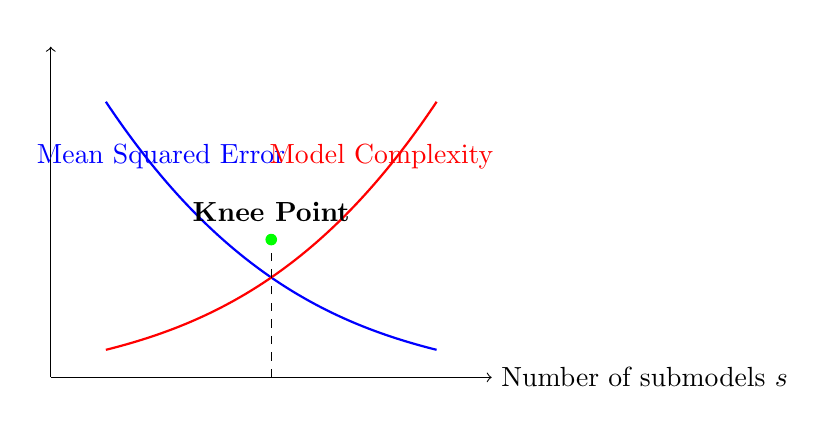
\begin{tikzpicture}[scale=0.7]
% Draw axes
\draw[->] (0,0) -- (8,0) node[right] {Number of submodels $s$};
\draw[->] (0,0) -- (0,6) node[above] {};

% Draw curves
\draw[thick, blue] (1,5) .. controls (3,2) and (5,1) .. (7,0.5);
\draw[thick, red] (1,0.5) .. controls (3,1) and (5,2) .. (7,5);

% Labels
\node[blue] at (2,4) {Mean Squared Error};
\node[red] at (6,4) {Model Complexity};
\node at (4,3) {\textbf{Knee Point}};
\draw[dashed] (4,0) -- (4,2.5);

% Add points
\fill[green] (4,2.5) circle (3pt);
\end{tikzpicture}
\end{center}

\textbf{Key Insight:} The optimal number of submodels is typically chosen at the "knee" of the complexity-accuracy trade-off curve.

\begin{alertblock}{MIN PFS Problem \cite{amaldi2002min}}
Find the minimum number $s$ of parameter vectors $\{\theta_i\}$ such that:
$$|y_k - \phi_k^T \theta_{\sigma(k)}| \leq \delta, \quad \forall k$$
for a given error bound $\delta > 0$.
\end{alertblock}
\end{frame}

\section{Modern Identification Approaches}

\begin{frame}{Modern Identification Landscape}
\begin{center}
\begin{tabular}{|l|l|l|l|}
\hline
\textbf{Method} & \textbf{Dynamics} & \textbf{Key Innovation} & \textbf{Paradigm} \\
\hline
\textbf{DAINARX} & Nonlinear NARX & Model fittability principle & Threshold-free \\
\textbf{FaMoS} & Linear ARX & Decision tree interpretability & Fast baseline \\
\textbf{LearnHA} & Polynomial ODEs & Handles resets & Complete HA learning \\
\textbf{HySynth} & Affine ODEs & $\epsilon$-capture guarantees & Online synthesis \\
\textbf{Classical (Paoletti)} & PWA/SARX & Four procedures survey & Foundation methods \\
\hline
\end{tabular}
\end{center}

\vspace{0.5cm}
\textbf{Canonical Identification Pipeline:}
\begin{enumerate}
\item \textcolor{blue}{Trace Segmentation} $\rightarrow$ partition data into mode segments
\item \textcolor{red}{Segment Clustering} $\rightarrow$ group segments by same dynamics
\item \textcolor{green}{Mode Characterization} $\rightarrow$ learn flow functions $F_q$
\item \textcolor{orange}{Guard/Reset Inference} $\rightarrow$ learn discrete transitions
\end{enumerate}

\begin{block}{Key Distinction}
\begin{itemize}
\item \textbf{Algebraic}: Focuses on SARX models (switching sequence estimation)
\item \textbf{Others}: Focus on PWARX models (polyhedral regions)
\end{itemize}
\end{block}
\end{frame}

\begin{frame}{The Evolution: From Heuristics to Principles}
\begin{columns}[t]
\begin{column}{0.5\textwidth}
\begin{block}{Traditional Heuristics}
\textbf{Derivative-based:}
\begin{itemize}
\item Detect "drastic variation"
\item User-defined thresholds
\item Noise sensitive
\end{itemize}

\textbf{Similarity-based:}
\begin{itemize}
\item Dynamic Time Warping
\item Signal shape comparison
\item Can misgroup dynamics
\end{itemize}
\end{block}
\end{column}
\begin{column}{0.5\textwidth}
\begin{block}{Modern Principles}
\textbf{Model Fittability:}
\begin{itemize}
\item Mathematical consistency
\item No arbitrary thresholds
\item Data-driven robustness
\end{itemize}

\textbf{Model Mergeability:}
\begin{itemize}
\item Test shared dynamics
\item Direct mathematical test
\item Formal guarantees
\end{itemize}
\end{block}
\end{column}
\end{columns}

\vspace{0.3cm}
\begin{alertblock}{Key Trend}
From fragile heuristics to robust mathematical principles.
\end{alertblock}
\end{frame}

\subsection{Classical Foundation: Paoletti et al.}

\begin{frame}{Classical Algebraic Procedure - Main Idea}
\begin{block}{Key Insight}
View identification of multiple ARX models as identification of a single "lifted" ARX model that encodes all submodels simultaneously.
\end{block}

\begin{block}{Hybrid Decoupling Constraint}
If data are generated by model with $s$ submodels, then:
$$\prod_{i=1}^s (b_i^T z_k) = 0, \quad \forall k$$
where $b_i = [1, \theta_i^T]^T$ and $z_k = [-y_k, \phi_k^T]^T$.
\end{block}

\begin{block}{Hybrid Decoupling Polynomial}
$$p_s(z) = \prod_{i=1}^s (b_i^T z) = h^T \nu_s(z)$$
where $\nu_s(z)$ contains all monomials of degree $s$ in $z$.
\end{block}

\textbf{Algorithm} \cite{vidal2003algebraic,ma2005identification}:
\begin{enumerate}
\item Solve linear system $L_s(K) h = 0$ to find $h$
\item Reconstruct parameter vectors using derivatives: $b_i = \frac{D p_s(z_{k_i})}{[1, 0, \ldots, 0] D p_s(z_{k_i})}$
\end{enumerate}
\end{frame}

\begin{frame}{Algebraic Procedure - Advantages \& Limitations}
\begin{columns}[t]
\begin{column}{0.5\textwidth}
\begin{block}{Advantages}
\begin{itemize}
\item Closed-form solution
\item No initialization required
\item Can estimate model orders
\item Can estimate number of submodels
\item Provably correct (noiseless case)
\end{itemize}
\end{block}

\begin{exampleblock}{Number of Submodels}
$$s = \arg\min\{i : \text{rank}(L_i(K)) = M_i(K) - 1\}$$
\end{exampleblock}
\end{column}
\begin{column}{0.5\textwidth}
\begin{block}{Limitations}
\begin{itemize}
\item Sensitive to noise
\item Only for SARX models
\item May not work with nonlinear disturbances
\item Classification may be suboptimal for PWARX
\end{itemize}
\end{block}

\begin{alertblock}{When to Use}
\begin{itemize}
\item System truly switched affine
\item Moderate noise levels
\item Unknown model structure
\item Need automatic model selection
\end{itemize}
\end{alertblock}
\end{column}
\end{columns}
\end{frame}

\subsection{Modern Threshold-Free: DAINARX}

\begin{frame}{DAINARX - Revolutionary Threshold-Free Approach}
\begin{block}{Key Innovation: Model Fittability Principle}
\textbf{Core Idea:} Replace subjective thresholds with objective mathematical consistency. A changepoint occurs when a growing data segment can no longer be explained by a single NARX model.
\end{block}

\textbf{DAINARX Pipeline:}
\begin{enumerate}
\item \textbf{Model Fittability Segmentation}: Detect changepoints when NARX model achieves near-zero error on growing window
\item \textbf{Model Mergeability Clustering}: Group segments that can be fit by same NARX instance
\item \textbf{Nonlinear Mode Learning}: Identify high-order NARX dynamics for each cluster
\item \textbf{Guard/Reset Inference}: Learn state-dependent switching conditions from transition data
\end{enumerate}

\begin{exampleblock}{Revolutionary Features}
\begin{itemize}
\item \textbf{Derivative-agnostic}: Works directly with sampled data
\item \textbf{Threshold-free}: No user-defined segmentation parameters
\item \textbf{High-order nonlinear}: Handles complex NARX dynamics
\item \textbf{Formal guarantees}: Mathematical consistency principles
\item \textbf{Complete HA}: Full hybrid automaton synthesis
\end{itemize}
\end{exampleblock}
\end{frame}

\begin{frame}{Clustering-based Procedure - Key Properties}
\begin{columns}[t]
\begin{column}{0.5\textwidth}
\begin{block}{Advantages}
\begin{itemize}
\item No prior knowledge needed
\item Single tuning parameter ($c$)
\item Can distinguish submodels with same parameters in different regions
\item Handles discontinuous dynamics
\end{itemize}
\end{block}

\begin{block}{Parameter $c$ Selection}
\begin{itemize}
\item Small $c$: Less noise filtering, fewer mixed datasets
\item Large $c$: More noise filtering, more mixed datasets
\item Trade-off between noise and purity
\end{itemize}
\end{block}
\end{column}
\begin{column}{0.5\textwidth}
\begin{block}{Limitations}
\begin{itemize}
\item Requires fixed $s$, $n_a$, $n_b$
\item Performance depends on ratio of mixed/pure local datasets
\item May fail with overestimated model orders
\end{itemize}
\end{block}

\begin{alertblock}{When to Use}
\begin{itemize}
\item No prior system knowledge
\item Prescribed model structure
\item Need to distinguish submodels in different regions
\end{itemize}
\end{alertblock}
\end{column}
\end{columns}

\vspace{0.3cm}
\begin{exampleblock}{Extension}
Modified version \cite{ferrari2003conditions} allows simultaneous estimation of number of submodels.
\end{exampleblock}
\end{frame}

\subsection{Fast Interpretable: FaMoS}

\begin{frame}{FaMoS - Fast Model Learning for CPS}
\begin{block}{Key Innovation: Decision Tree Representation}
\textbf{Goal:} Fast identification of linear ARX dynamics with human-interpretable switching logic represented as decision trees.
\end{block}

\textbf{FaMoS Key Features:}
\begin{itemize}
\item High-order linear ARX dynamics
\item Decision tree switching logic
\item Fast baseline for hybrid CPS
\item Human-interpretable structure
\item Scalable to industrial systems
\end{itemize}

\begin{block}{Classification Rule}
$$\sigma(k) = i^* \quad \text{where } i^* = \arg\max_{i=1,\ldots,s} p((y_k, r_k) | \sigma(k) = i)$$
\end{block}

\begin{block}{Bayes Update}
$$p_{\theta_{i^*}}(\theta; k) = \frac{p((y_k, r_k) | \theta) p_{\theta_{i^*}}(\theta; k-1)}{\int_{\Theta_{i^*}} p((y_k, r_k) | \tilde{\theta}) p_{\theta_{i^*}}(\tilde{\theta}; k-1) d\tilde{\theta}}$$
\end{block}
\end{frame}

\begin{frame}{Bayesian Procedure - Advanced Features}
\begin{block}{Likelihood Function}
$$p((y_k, r_k) | \theta) = p_e(y_k - \theta^T \phi_k)$$
where $p_e(\cdot)$ is the pdf of the noise term.
\end{block}

\begin{block}{Misclassification Weights for Region Estimation}
For data point $(y_k, r_k)$ attributed to mode $i$, the price for misclassification into mode $j$ is:
$$\nu_{i,j}(r_k) = \log \frac{p((y_k, r_k) | \sigma(k) = i)}{p((y_k, r_k) | \sigma(k) = j)}$$
\end{block}

\textbf{Implementation:}
\begin{itemize}
\item Particle filtering algorithms for numerical implementation
\item Modified Multicategory RLP (MRLP) for region estimation
\item Automatic weight computation reduces misclassification penalties
\end{itemize}

\begin{alertblock}{Key Feature}
Zero misclassification price when probabilities are equal!
\end{alertblock}
\end{frame}

\begin{frame}{Bayesian Procedure - Evaluation}
\begin{columns}[t]
\begin{column}{0.5\textwidth}
\begin{block}{Advantages}
\begin{itemize}
\item Incorporates prior knowledge naturally
\item Automatic misclassification weights
\item Probabilistic framework
\item Various parameter estimates available (MAP, expectation)
\end{itemize}
\end{block}

\begin{exampleblock}{Applications}
Successfully applied to:
\begin{itemize}
\item Pick-and-place machines \cite{juloski2004data}
\item Industrial process control
\item Systems with known physical modes
\end{itemize}
\end{exampleblock}
\end{column}
\begin{column}{0.5\textwidth}
\begin{block}{Limitations}
\begin{itemize}
\item Requires fixed $s$, $n_a$, $n_b$
\item Sensitive to initialization
\item Requires specification of prior pdfs
\item Computational complexity with particle filters
\end{itemize}
\end{block}

\begin{alertblock}{When to Use}
\begin{itemize}
\item Prior knowledge available
\item Physical insight into system modes
\item Need probabilistic uncertainty quantification
\item Can tolerate computational cost
\end{itemize}
\end{alertblock}
\end{column}
\end{columns}

\vspace{0.3cm}
\begin{block}{Tuning Parameters}
Most critical: Prior pdfs $p_{\theta_i}(\cdot; 0)$ and noise pdf $p_e(\cdot)$
\end{block}
\end{frame}

\subsection{Complete HA Learning: LearnHA}

\begin{frame}{LearnHA - Complete Hybrid Automata Learning}
\begin{block}{Key Innovation: Full HA Synthesis}
\textbf{Capability:} Learn complete hybrid automata with polynomial ODEs, including external inputs and state resets - features often missing from other frameworks.
\end{block}

\textbf{LearnHA Capabilities:}
\begin{itemize}
\item First-order polynomial ODEs
\item External input handling
\item Linear state resets
\item Complete hybrid automaton synthesis
\item DTW-based segment clustering
\end{itemize}

\begin{block}{Parameter Estimation}
$$\theta_i = \arg\min_\theta \max_{(y_k,r_k) \in D_i} |y_k - \phi_k^T \theta|$$
($\ell_\infty$ projection estimator)
\end{block}
\end{frame}

\begin{frame}{Bounded-error Procedure - Model Reduction}
\begin{block}{Submodel Merging}
Merge submodels $i$ and $j$ if:
$$\alpha_{i,j} = \frac{\|\theta_i - \theta_j\|}{\min\{\|\theta_i\|, \|\theta_j\|\}} < \alpha$$
\end{block}

\begin{block}{Submodel Removal}
Remove submodel $i$ if cardinality of data set $D_i$ is less than $\beta N$.
\end{block}

\begin{alertblock}{Outlier Detection}
Data points that cannot satisfy the bound $\delta$ are automatically discarded during classification, enabling outlier detection.
\end{alertblock}

\textbf{Multi-output Extension:}
$$\|y_k - f(r_k)\|_\infty \leq \delta, \quad \forall k$$
\end{frame}

\begin{frame}{Bounded-error Procedure - Evaluation}
\begin{columns}[t]
\begin{column}{0.5\textwidth}
\begin{block}{Advantages}
\begin{itemize}
\item Prescribed accuracy through $\delta$
\item Automatic outlier detection
\item Model complexity control
\item No prior knowledge needed
\item Multi-output capability
\end{itemize}
\end{block}

\begin{exampleblock}{Trade-off Control}
\begin{itemize}
\item Smaller $\delta$ $\rightarrow$ more submodels, better fit
\item Larger $\delta$ $\rightarrow$ fewer submodels, worse fit
\end{itemize}
\end{exampleblock}
\end{column}
\begin{column}{0.5\textwidth}
\begin{block}{Limitations}
\begin{itemize}
\item Requires fixed $n_a$, $n_b$
\item Suboptimal MIN PFS solution
\item Multiple tuning parameters
\item May need several attempts for good results
\end{itemize}
\end{block}

\begin{alertblock}{When to Use}
\begin{itemize}
\item Need prescribed accuracy
\item Presence of outliers
\item Approximating nonlinear dynamics
\item Multi-output systems
\end{itemize}
\end{alertblock}
\end{column}
\end{columns}

\vspace{0.3cm}
\begin{block}{Main Tuning Parameter}
$\delta$: Controls accuracy-complexity trade-off. Optional: $\alpha$, $\beta$ for model reduction.
\end{block}
\end{frame}

\begin{frame}{Comprehensive Method Comparison}
\vspace{-0.3cm}
\begin{center}
\scriptsize
\begin{tabular}{|l|l|l|c|c|c|l|}
\hline
\textbf{Method} & \textbf{Dynamics} & \textbf{Scope} & \textbf{H.O.} & \textbf{Reset} & \textbf{Input} & \textbf{Key Feature} \\
\hline
\textbf{DAINARX} & Nonlinear NARX & HA & Y & Y & Y & Threshold-free \\
\textbf{FaMoS} & Linear ARX & HA & Y & N & Y & Decision trees \\
\textbf{LearnHA} & Polynomial & HA & N & Y & Y & Complete HA \\
\textbf{HySynth} & Affine & HA & N & N & N & $\epsilon$-capture \\
\textbf{Classical} & PWA/Linear & SA & ± & ± & ± & Foundation \\
\hline
\end{tabular}
\end{center}

\vspace{0.2cm}
\begin{alertblock}{Trade-off Insight}
\textbf{Expressiveness vs. Tractability:} Linear methods are fast but limited. Nonlinear methods are powerful but require more assumptions.
\end{alertblock}
\end{frame}

\section{Data Classification and Region Estimation}

\begin{frame}{The Classification Challenge}
\begin{center}
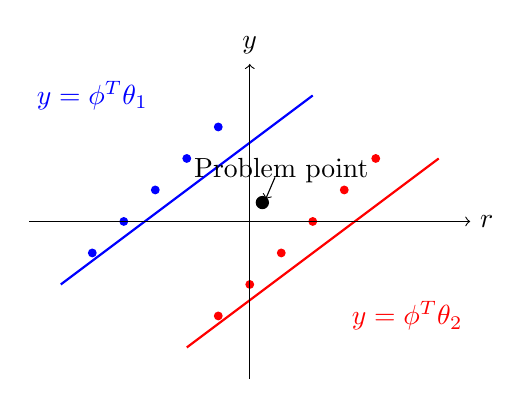
\begin{tikzpicture}[scale=0.8]
% Draw two intersecting lines
\draw[thick, blue] (-3,-1) -- (1,2);
\draw[thick, red] (-1,-2) -- (3,1);

% Draw data points
\foreach \x/\y in {-2.5/-0.5, -2/0, -1.5/0.5, -1/1, -0.5/1.5} {
    \fill[blue] (\x,\y) circle (2pt);
}
\foreach \x/\y in {-0.5/-1.5, 0/-1, 0.5/-0.5, 1/0, 1.5/0.5, 2/1} {
    \fill[red] (\x,\y) circle (2pt);
}

% Problem point
\fill[black] (0.2,0.3) circle (3pt);
\node at (0.5, 0.8) {Problem point};
\draw[->] (0.4, 0.7) -- (0.25, 0.35);

% Labels
\node[blue] at (-2.5, 2) {$y = \phi^T\theta_1$};
\node[red] at (2.5, -1.5) {$y = \phi^T\theta_2$};

% Draw axes
\draw[->] (-3.5,0) -- (3.5,0) node[right] {$r$};
\draw[->] (0,-2.5) -- (0,2.5) node[above] {$y$};
\end{tikzpicture}
\end{center}

\begin{alertblock}{Intersecting Submodels Problem}
Data points near submodel intersections can be assigned to either submodel, leading to:
\begin{itemize}
\item Wrong data attribution
\item Non-linearly separable clusters
\item Poor region estimation
\end{itemize}
\end{alertblock}

\textbf{Solutions in the Four Procedures:}
\begin{itemize}
\item \textbf{Bounded-error}: Undecidable points with refinement procedure
\item \textbf{Bayesian}: Misclassification weights based on likelihood ratios
\item \textbf{Clustering}: Clustering in feature space with confidence measures
\end{itemize}
\end{frame}

\begin{frame}{Linear Separation Techniques}
After data classification, we need to estimate polyhedral regions. Two approaches:

\begin{columns}[t]
\begin{column}{0.5\textwidth}
\begin{block}{Pairwise Separation}
For each pair $(A_i, A_j)$ of data clusters, find hyperplane:
$$w^T r_k + \gamma > 0, \quad \forall r_k \in A_i$$
$$w^T r_k + \gamma < 0, \quad \forall r_k \in A_j$$

\textbf{Advantages:}
\begin{itemize}
\item Computationally efficient
\item Parallelizable
\end{itemize}

\textbf{Disadvantages:}
\begin{itemize}
\item May create holes in partition
\item Not guaranteed to be complete
\end{itemize}
\end{block}
\end{column}
\begin{column}{0.5\textwidth}
\begin{block}{Multi-class Separation}
Find $s$ classification functions simultaneously such that class $i$ function is maximal for data in $A_i$.

\textbf{Methods:}
\begin{itemize}
\item Multi-category SVM (M-SVM) \cite{cortes1995support}
\item Multi-category RLP (M-RLP) \cite{bennett1992robust}
\end{itemize}

\textbf{Advantages:}
\begin{itemize}
\item Guaranteed complete partition
\item Global optimality
\end{itemize}

\textbf{Disadvantages:}
\begin{itemize}
\item Higher computational cost
\item All data processed simultaneously
\end{itemize}
\end{block}
\end{column}
\end{columns}
\end{frame}

\begin{frame}{Handling Non-separable Data}
\begin{block}{Robust Linear Programming (RLP)}
When data are not linearly separable:
\begin{align}
\min_{w,\gamma,v_k} &\quad \sum_k c_k v_k \\
\text{s.t.} \quad &z_k[w^T r_k + \gamma] \geq 1 - v_k \\
&v_k \geq 0, \quad \forall k
\end{align}
where $z_k = 1$ if $r_k \in A_i$, $z_k = -1$ if $r_k \in A_j$.
\end{block}

\begin{itemize}
\item $v_k$: slack variables (misclassification errors)
\item $c_k$: misclassification weights (can be adaptive)
\item Reduces to standard SVM with quadratic objective
\end{itemize}

\begin{exampleblock}{Bayesian Extension}
In Bayesian procedure: $c_k = \nu_{i,j}(r_k) = \log\frac{p((y_k,r_k)|\sigma(k)=i)}{p((y_k,r_k)|\sigma(k)=j)}$
\end{exampleblock}
\end{frame}

\section{Recent Advances (2020-2024)}

\begin{frame}{Recent Advances in Hybrid System Identification}
\begin{block}{Methodological Maturation}
\textbf{From Heuristics to Principles:}
\begin{itemize}
\item \textbf{Traditional}: Derivative variation, signal similarity (DTW), user thresholds
\item \textbf{Modern}: Model fittability principle, mathematical consistency
\item \textbf{Benefits}: Robustness, formal guarantees, reduced manual tuning
\item \textbf{Challenge}: Computational complexity, template requirements
\end{itemize}
\end{block}

\begin{block}{Integration with Modern ML}
\textbf{Deep Learning Opportunities:}
\begin{itemize}
\item Neural networks for complex flow dynamics approximation
\item Foundation models pre-trained on diverse physical systems
\item Transfer learning for CPS-specific fine-tuning
\item Grey-box modeling: interpretability + expressiveness
\end{itemize}
\end{block}

\begin{block}{Online and Adaptive Methods}
\textbf{Real-time Identification:}
\begin{itemize}
\item Online identification using integral concurrent learning \cite{yang2021online}
\item Active mode recognition algorithms
\item Distributed identification strategies \cite{chen2021piecewise}
\item Recursive methods with automatic tuning
\end{itemize}
\end{block}

\begin{alertblock}{Key Trend}
Integration of classical hybrid system identification with modern machine learning to leverage both interpretability and approximation power.
\end{alertblock}
\end{frame}

\begin{frame}{Neural Network-Based PWA Identification}
\begin{block}{Variational Autoencoder Approach}
\textbf{Key Idea:} Use VAE with specialized structure where:
\begin{itemize}
\item \textcolor{blue}{Encoder}: Provides categorical latent variables representing discrete modes
\item \textcolor{red}{Decoder}: Set of neural networks, each corresponding to a local submodel
\item \textcolor{green}{Latent space}: Interpretable representation of hybrid system modes
\end{itemize}
\end{block}

\begin{center}
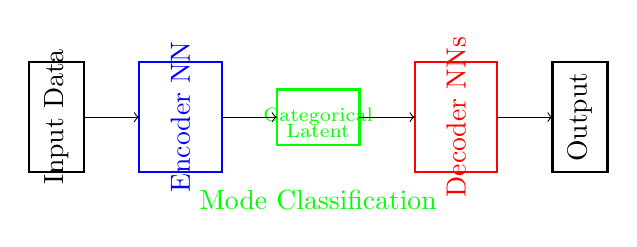
\begin{tikzpicture}[scale=0.7]
% Input
\draw[thick] (0,0) rectangle (1,2);
\node at (0.5,1) {\rotatebox{90}{Input Data}};

% Encoder
\draw[thick, blue] (2,0) rectangle (3.5,2);
\node[blue] at (2.75,1) {\rotatebox{90}{Encoder NN}};

% Latent space
\draw[thick, green] (4.5,0.5) rectangle (6,1.5);
\node[green] at (5.25,1) {\scriptsize Categorical};
\node[green] at (5.25,0.75) {\scriptsize Latent};

% Decoder
\draw[thick, red] (7,0) rectangle (8.5,2);
\node[red] at (7.75,1) {\rotatebox{90}{Decoder NNs}};

% Output
\draw[thick] (9.5,0) rectangle (10.5,2);
\node at (10,1) {\rotatebox{90}{Output}};

% Arrows
\draw[->] (1,1) -- (2,1);
\draw[->] (3.5,1) -- (4.5,1);
\draw[->] (6,1) -- (7,1);
\draw[->] (8.5,1) -- (9.5,1);

\node at (5.25, -0.5) {\textcolor{green}{Mode Classification}};
\end{tikzpicture}
\end{center}

\textbf{Advantages:}
\begin{itemize}
\item Automatic feature learning
\item Joint mode classification and parameter estimation
\item Scalable to high-dimensional systems
\end{itemize}
\end{frame}

\begin{frame}{PWA Decomposition of Neural Networks}
\begin{block}{Reverse Problem}
\textbf{Objective:} Given a trained neural network, compute a low-complexity PWA function that closely approximates it.
\end{block}

\begin{exampleblock}{F-16 Jet Benchmark}
Successfully demonstrated on nonlinear system identification benchmark using F-16 aircraft data:
\begin{itemize}
\item Original neural network: High complexity, black-box
\item PWA approximation: Interpretable, suitable for controller synthesis
\item Performance: Maintains approximation accuracy with reduced complexity
\end{itemize}
\end{exampleblock}

\textbf{Benefits:}
\begin{itemize}
\item Combines machine learning applicability with PWA controller synthesis
\item Interpretable approximation of neural network decisions
\item Enables formal verification and analysis
\item Suitable for safety-critical applications
\end{itemize}

\begin{alertblock}{Impact}
Bridges the gap between powerful neural network approximation and the need for interpretable, analyzable models in control systems.
\end{alertblock}
\end{frame}

\begin{frame}{Online and Distributed Identification}
\begin{block}{Online Identification Challenges}
\textbf{Requirements:}
\begin{itemize}
\item Real-time parameter adaptation
\item Active mode recognition during operation
\item Handling of unknown switching sequences
\item Computational efficiency for embedded systems
\end{itemize}
\end{block}

\begin{block}{Recent Solutions}
\textbf{Integral Concurrent Learning} \cite{yang2021online}:
\begin{itemize}
\item Online estimation of continuous-time PWA systems
\item Simultaneous identification of: number of subsystems, switching sequence, parameters
\item Concurrent learning identifiers with theoretical guarantees
\end{itemize}

\textbf{Distributed Identification:}
\begin{itemize}
\item Centralized vs. distributed parameter estimation \cite{chen2021piecewise}
\item Network-based identification for large-scale systems
\item Hierarchical approaches using gap metric clustering \cite{lu2020pwa}
\end{itemize}
\end{block}

\begin{exampleblock}{Applications}
Industrial process control, automotive systems, smart grid management
\end{exampleblock}
\end{frame}

\section{Practical Guidelines and Applications}

\begin{frame}{Method Selection Guidelines}
\vspace{-0.2cm}
\begin{center}
\small
\begin{tabular}{|l|l|l|l|}
\hline
\textbf{Scenario} & \textbf{Method} & \textbf{Advantage} & \textbf{Limitation} \\
\hline
Unknown structure & DAINARX & Threshold-free & Template needed \\
Fast interpretable & FaMoS & Decision trees & Linear only \\
Complete HA needed & LearnHA & Resets \& inputs & First-order \\
Online learning & HySynth & $\epsilon$-guarantees & Affine only \\
Clean classical data & Algebraic & Closed-form & Noise sensitive \\
\hline
\end{tabular}
\end{center}

\vspace{0.3cm}
\begin{alertblock}{Hybrid Approach}
Combine methods: e.g., Classical initialization + Modern refinement
\end{alertblock}
\end{frame}

\begin{frame}{Real-world Applications}
\begin{columns}[t]
\begin{column}{0.5\textwidth}
\begin{block}{Industrial CPS}
\textbf{Pick-and-place:} \cite{juloski2004data}
\begin{itemize}
\item Electronic component placement
\item Multiple operating modes
\end{itemize}

\textbf{Automotive:} \cite{borrelli2006mpc}
\begin{itemize}
\item Traction control systems
\item Engine/transmission control
\end{itemize}
\end{block}
\end{column}
\begin{column}{0.5\textwidth}
\begin{block}{Other Domains}
\textbf{Computer Vision:}
\begin{itemize}
\item Motion segmentation
\item Video analysis
\end{itemize}

\textbf{Biology:} \cite{ferrari2007hybrid}
\begin{itemize}
\item Gene regulatory networks
\item Metabolic pathways
\end{itemize}
\end{block}
\end{column}
\end{columns}

\vspace{0.3cm}
\begin{exampleblock}{Success Factors}
Proper method selection, careful tuning, validation, domain expertise integration.
\end{exampleblock}
\end{frame}

\section{Grand Challenges and Future Directions}

\begin{frame}{Grand Challenges from the Survey}
\begin{block}{The Noise and Uncertainty Problem}
\begin{itemize}
\item Most methods assume clean, noise-free data
\item Real sensors have errors and disturbances
\item Noise creates spurious mode switches
\item Need robust methods with noise modeling
\end{itemize}
\end{block}

\begin{block}{The Template Conundrum}
\begin{itemize}
\item Advanced methods require user-provided templates
\item Contradicts "black-box" identification premise
\item Need automatic structure discovery
\item Goal: Fully automated model learning
\end{itemize}
\end{block}

\begin{block}{Scalability and Formal Guarantees}
\begin{itemize}
\item \textbf{Curse of dimensionality}: Industrial CPS with dozens of variables/modes
\item \textbf{Polynomial complexity}: DAINARX polynomial but high-degree in practice
\item \textbf{Formal guarantees}: Need PAC learning bounds on model quality
\item \textbf{Goal}: Certifiably safe CPS from learned components
\end{itemize}
\end{block}

\begin{alertblock}{Fundamental Trade-offs}
\begin{itemize}
\item \textbf{Accuracy vs. Complexity}: More submodels improve fit but risk overfitting
\item \textbf{Interpretability vs. Performance}: Neural approaches vs. classical methods
\item \textbf{Generality vs. Efficiency}: Universal methods vs. domain-specific approaches
\end{itemize}
\end{alertblock}
\end{frame}

\begin{frame}{Future Research Directions}
\begin{block}{Deep Learning Integration}
\begin{itemize}
\item Neural networks enable arbitrary nonlinearities
\item Black-box nature conflicts with verification
\item Requires massive datasets
\item Solution: Hybrid interpretable approaches
\end{itemize}
\end{block}

\begin{block}{Foundation Models \& Digital Twins}
\begin{itemize}
\item Pre-trained on diverse physical systems
\item Fine-tune with small CPS datasets
\item Grey-box modeling paradigm
\item High-fidelity digital replicas
\end{itemize}
\end{block}

\begin{block}{Theoretical Development}
\begin{itemize}
\item Persistence of excitation for hybrid systems
\item Identifiability conditions for PWA models
\item Sample complexity analysis for different methods
\item Robustness guarantees for identified models
\end{itemize}
\end{block}
\end{frame}

\begin{frame}{Open Problems}
\begin{enumerate}
\item \textbf{Optimal input design}: How to design experiments that maximize information for hybrid system identification?

\item \textbf{High-dimensional systems}: Scalable methods for systems with hundreds of states and inputs?

\item \textbf{Distributed identification}: How to identify large-scale networked hybrid systems?

\item \textbf{Safety and verification}: How to ensure identified models are safe for control applications?

\item \textbf{Online adaptation}: How to continuously adapt models as system behavior changes?

\item \textbf{Multi-modal data}: Integration of different data types (time series, images, text) for hybrid system identification?
\end{enumerate}

\begin{alertblock}{Ultimate Vision: Push-Button Synthesis}
\textbf{Goal:} Raw noisy sensor data $\rightarrow$ Formal hybrid automaton with verifiable safety guarantees. \textbf{Requires:} Synthesis of DAINARX principles + PAC learning theory + automated verification.
\end{alertblock}
\end{frame}

\section{Conclusion}

\begin{frame}{Summary}
\begin{block}{Key Takeaways}
\begin{itemize}
\item \textbf{CPS imperative}: "Model-first" engineering creates "learn-first" necessity for safety-critical systems
\item \textbf{Methodological evolution}: From fragile heuristics to robust mathematical principles
\item \textbf{Modern state-of-art}: DAINARX (threshold-free), FaMoS (interpretable), LearnHA (complete)
\item \textbf{Future integration}: Foundation models + formal verification for automated CPS design
\end{itemize}
\end{block}

\begin{block}{Evolution Timeline}
\begin{enumerate}
\item \textcolor{blue}{\textbf{Classical Foundation (2007)}}: Paoletti et al. four procedures, PWA/SARX focus
\item \textcolor{red}{\textbf{Threshold-Free Revolution}}: DAINARX model fittability principle
\item \textcolor{green}{\textbf{Specialized Methods}}: FaMoS (speed), LearnHA (completeness), HySynth (guarantees)
\item \textcolor{orange}{\textbf{Future Vision}}: Foundation models + automated verification
\end{enumerate}
\end{block}

\begin{exampleblock}{Critical Research Gaps}
\textbf{Laboratory vs. Industry:} Current methods excel on clean, simulated data but struggle with noisy industrial sensors, high-dimensional systems, and unknown structures. Bridging this gap is essential for CPS deployment.
\end{exampleblock}
\end{frame}

\begin{frame}{Thank You - Questions?}
\begin{center}
\Large{Questions and Discussion}
\end{center}

\vspace{1cm}

\begin{block}{Further Reading}
\textbf{Classical Reference:}
\begin{itemize}
\item \cite{paoletti2007identification}
\end{itemize}

\textbf{Recent Surveys:}
\begin{itemize}
\item \cite{lauer2023models}
\item \cite{chen2024deep}
\end{itemize}

\textbf{Software Tools:}
\begin{itemize}
\item Hybrid Identification Toolbox (HIT) - Ferrari-Trecate
\item Various implementations available on GitHub
\end{itemize}
\end{block}

\begin{center}
\textbf{Contact:} Workshop on Automata Learning
\end{center}
\end{frame}

% Bibliography
\begin{frame}[allowframebreaks]{References}
\printbibliography
\end{frame}

\end{document}